\chapter{Performance Evaluation}
\label{cha:evaluation}

Answering the question of GC performance under a real-world setting,
this chapter discusses the performance evaluation I undertook for analyzing
the Garbage-first family of garbage collectors.
This chapter will first describe the software and hardware platform I used for benchmarking.
Then the detailed evaluation process and results of pause time,
concurrency overhead, and remembered-set footprint will be presented and discussed.

Section~\ref{sec:dacapo} and \ref{sec:hardware} introduce the experimental
platform and software involved for the performance measurements.
Section~\ref{sec:generalmethod} discusses the general evaluation method used to
evaluate the performance of all the interested metrics.
Section~\ref{sec:pausetime}, \ref{sec:barrierlatency} and \ref{sec:remsetsize} discusses the detailed
measurement steps involved to evaluate the GC pause time, concurrency overhead and remembered set size
respectively, as well
as figures of the results and the resulting discussions.

\section{The DaCapo Benchmarks} % 2
\label{sec:dacapo}

The DaCapo Benchmark Suite is a tool for Java benchmarking and contains a set of
open-sourced real-world programs with a high memory load.

The DaCapo benchmarks are frequently used during the development of the G1 family
of garbage collectors in Chapter~\ref{cha:implementation}, as a validation program
to verify the correctness of the collectors under a real-world setting.

I also performed pause time evaluations and concurrency overhead evaluation
on all of the following DaCapo Benchmark suites.
The benchmarking suites I used for evaluation includes \citep{Blackburn:2006:DBJ:1167515.1167488}:

\begin{itemize}
  \item \textbf{antlr} Parses one or more grammar files and generates a parser and lexical analyzer for each.
  \item \textbf{luindex} Uses lucene to indexes a set of documents; the works of Shakespeare and the King James Bible.
  \item \textbf{bloat} Performs a number of optimizations and analysis on Java bytecode files.
  \item \textbf{hsqldb} Executes a JDBCbench-like in-memory benchmark, executing a number of transactions against a model of a banking application.
  \item \textbf{lusearch} Uses lucene to do a text search of keywords over a corpus of data comprising the works of Shakespeare and the King James Bible.
  \item \textbf{pmd} Analyzes a set of Java classes for a range of source code problems.
  \item \textbf{xalan} Transforms XML documents into HTML.
  \item \textbf{eclipse} executes some of the (non-gui) jdt performance tests for the Eclipse IDE.
  \item \textbf{avrora} Simulates a number of programs run on a grid of AVR microcontrollers.
  \item \textbf{sunflow} Renders a set of images using ray tracing.
\end{itemize}

Except \textit{antlr}, \textit{eclipse}, \textit{fop}, \textit{hsqldb} and \textit{pmd} are coming from
DaCapo 2006, all the other benchmarks are coming from the DaCapo version 9.12.
Some of the implemented G1 family of collectors can cause some bugs when running on
\textit{tomcat}, \textit{batik} and \textit{bloat} benchmarks so I did not include
these benchmarks when performing measurements.

By performing evaluations on a wide range of benchmarking suites which represents different
class of real-world programs, it is more possible to understand the pros and cons
of the G1 family of collectors under a real-world setting.

\section{Hardware Platform} % 2
\label{sec:hardware}

During the implementation and evaluation of all the G1 family of garbage collectors in Chapter~\ref{cha:implementation},
a list of machines with a variety on CPU types, clock, number of processors and
the size of cache and memory were involved, as shown in Table~\ref{tab:machines}.

As part of the implementation process,
by executing the benchmarks on these different machines,
% and thanks to the benchmarking suites of the DaCapo Benchmark which reflect
% different categories of programs in the real world,
I have the ability to statistically verify the correctness of the previously
implemented garbage collectors (in Chapter~\ref{cha:implementation})
and make sure they perform as intended in a real-world setting.

For further performance evaluation, the "fisher" machine was used for the final benchmarking.

\begin{table*}
  \centering
  \input table/machines.tex
  \caption{Machines used for development and evaluation.}
  \label{tab:machines}
\end{table*}

\section{General Measurement Methodology}
\label{sec:generalmethod}

I perform both GC pause time and concurrency overhead measurements on the optimized build
of the JikesRVM, with 6 different builds for the 6 GCs to be measured respectively.
To collect measurement results, I executed all 10 DaCapo benchmarks discussed in Section~\ref{sec:dacapo}
on all 6 collectors, with respect to 4 different heap sizes, 637\,MB, 939\,MB, 1414\,MB, and 1971\,MB
respectively. This is abnormal since usually heap sizes are different for each benchmark. But by using difference
heap sizes for difference benchmarks, it is meaningless to evaluate and compare
GC pause time over different heap sizes. So in this thesis I assign each benchmark the
same heap size so that I can later compare GC pause time among difference collectors when
targeting the same heap size.

Each benchmark suite is executed 10 times for each configuration of $(GC, HeapSize)$ to
collect more precise results and avoid the error due to some unexpected environmental fluctuations.

\subsection{Reducing non-determinisms}
\label{subsec:nondeterminisms}

The adaptive compiler can have non-deterministic behaviors when performing dynamic
compilations and optimizations to the executing Java program. In order to minimize
such non-deterministic behaviors and make the program execute faster, I performed
the measurement methodology called "warmup replay", which was firstly introduced by
\cite{yang2012barriers}, as a replacement of the "pseudoadaptive approach" introduced by \cite{blackburn2004barriers}.

This methodology performs an execution of 10 iterations for each benchmark suite to
collect run time execution information before the measurement, to assist with more optimized compilation.
Then during measurements, after the first iteration of warmups, JikesRVM compiles all
methods with the advice information generated previously to avoid any re-compilation
behaviors during the following measurement iteration.

I ran all of the 10 benchmark suites discussed in Section~\ref{sec:dacapo} on each collector
for 10 times, with 2 times of warmup execution before the timing iteration.
JikesRVM performs warmup-replay compilation at the end of the first warmup iteration.

\section{Pause Time Evaluation} % 7
\label{sec:pausetime}

This section describes the steps took for pause time evaluation as well as
all the evaluation results and discussions.

\subsection{Mutator latency timer}

In order to perform more careful analysis on the mutator pause times, instead of
simply calculating the time starting from the first stop-the-world phase to the last
stop-the-world phase during each GC cycle, I implemented a mutator latency timer
to perform a more precise calculation of mutator pause times.

The mutator latency timer contains a static "three-dimensional" array:\\
\centerline{\textjava{static long[] LOGS = long[THREAD_ID * EVENT_ID * NUM_LOGS]}}
This array is statically allocated within the VM Space to record the timestamp (in nanoseconds)
of each event and each mutator. The first dimension is the thread id of all
mutators. The second dimension is the event id. The third dimensional \textjava{NUM_LOGS} is the
max number of logs of one $(event_id, event_id)$ combination and is currently set to $1024$. Particularly under
the current context, to measure the pause time for each mutator, two events,
\textjava{MUTATOR_PAUSE} and \textjava{MUTATOR_RESUME} are defined to record the time when a
mutator thread starts waiting for GC complete and the time when a mutator gets resumed from a GC pause for execution.

In JikesRVM, every time the program reaches a yieldpoint, the mutator
thread checks for GC requests and starts waiting if necessary , which will trigger a \textjava{MUTATOR_PAUSE} event if it should
be paused. After a stop-the-world cycle is finished, before continuing for further execution,
it triggers a \textjava{MUTATOR_RESUME} event immediately after gets resumed

At the end of the benchmark execution, the mutator latency timer will dump all the
data in the \textjava{LOGS} array to the print buffer for further data analysis.

As an output of the analysis of the overhead data, I report the minimum, 50\%,
and 95 percentile mutator pause time for each GC, each benchmark suite and each heap size.

\subsection{MMTk harness callbacks}

During each iteration of benchmarking, the DaCapo benchmark has several warm-up
executions which will run the benchmark suite a few times to warm up the cache and JVM.
Then the DaCapo benchmark will start the actual benchmarking run. I use a probe called \textjava{MMTKCallback}
which will call the \textjava{org.mmtk.plan.Plan.harnessBegin} method
before the start of the final benchmarking execution and call the \textjava{org.mmtk.plan.Plan.harnessEnd}
after the final benchmarking execution. Based on this, the two callbacks
\textjava{harnessBegin} and \textjava{harnessEnd} are used to calculate the inform the mutator
latency timer to start recording logs or dump all recorded logs.

\subsection{Results}

\begin{table*}
  \centering
  \input table/average-pause.tex
  \caption{Results of the GC pause time}
  \label{tab:pause}
\end{table*}

\begin{figure*}
  \centering
  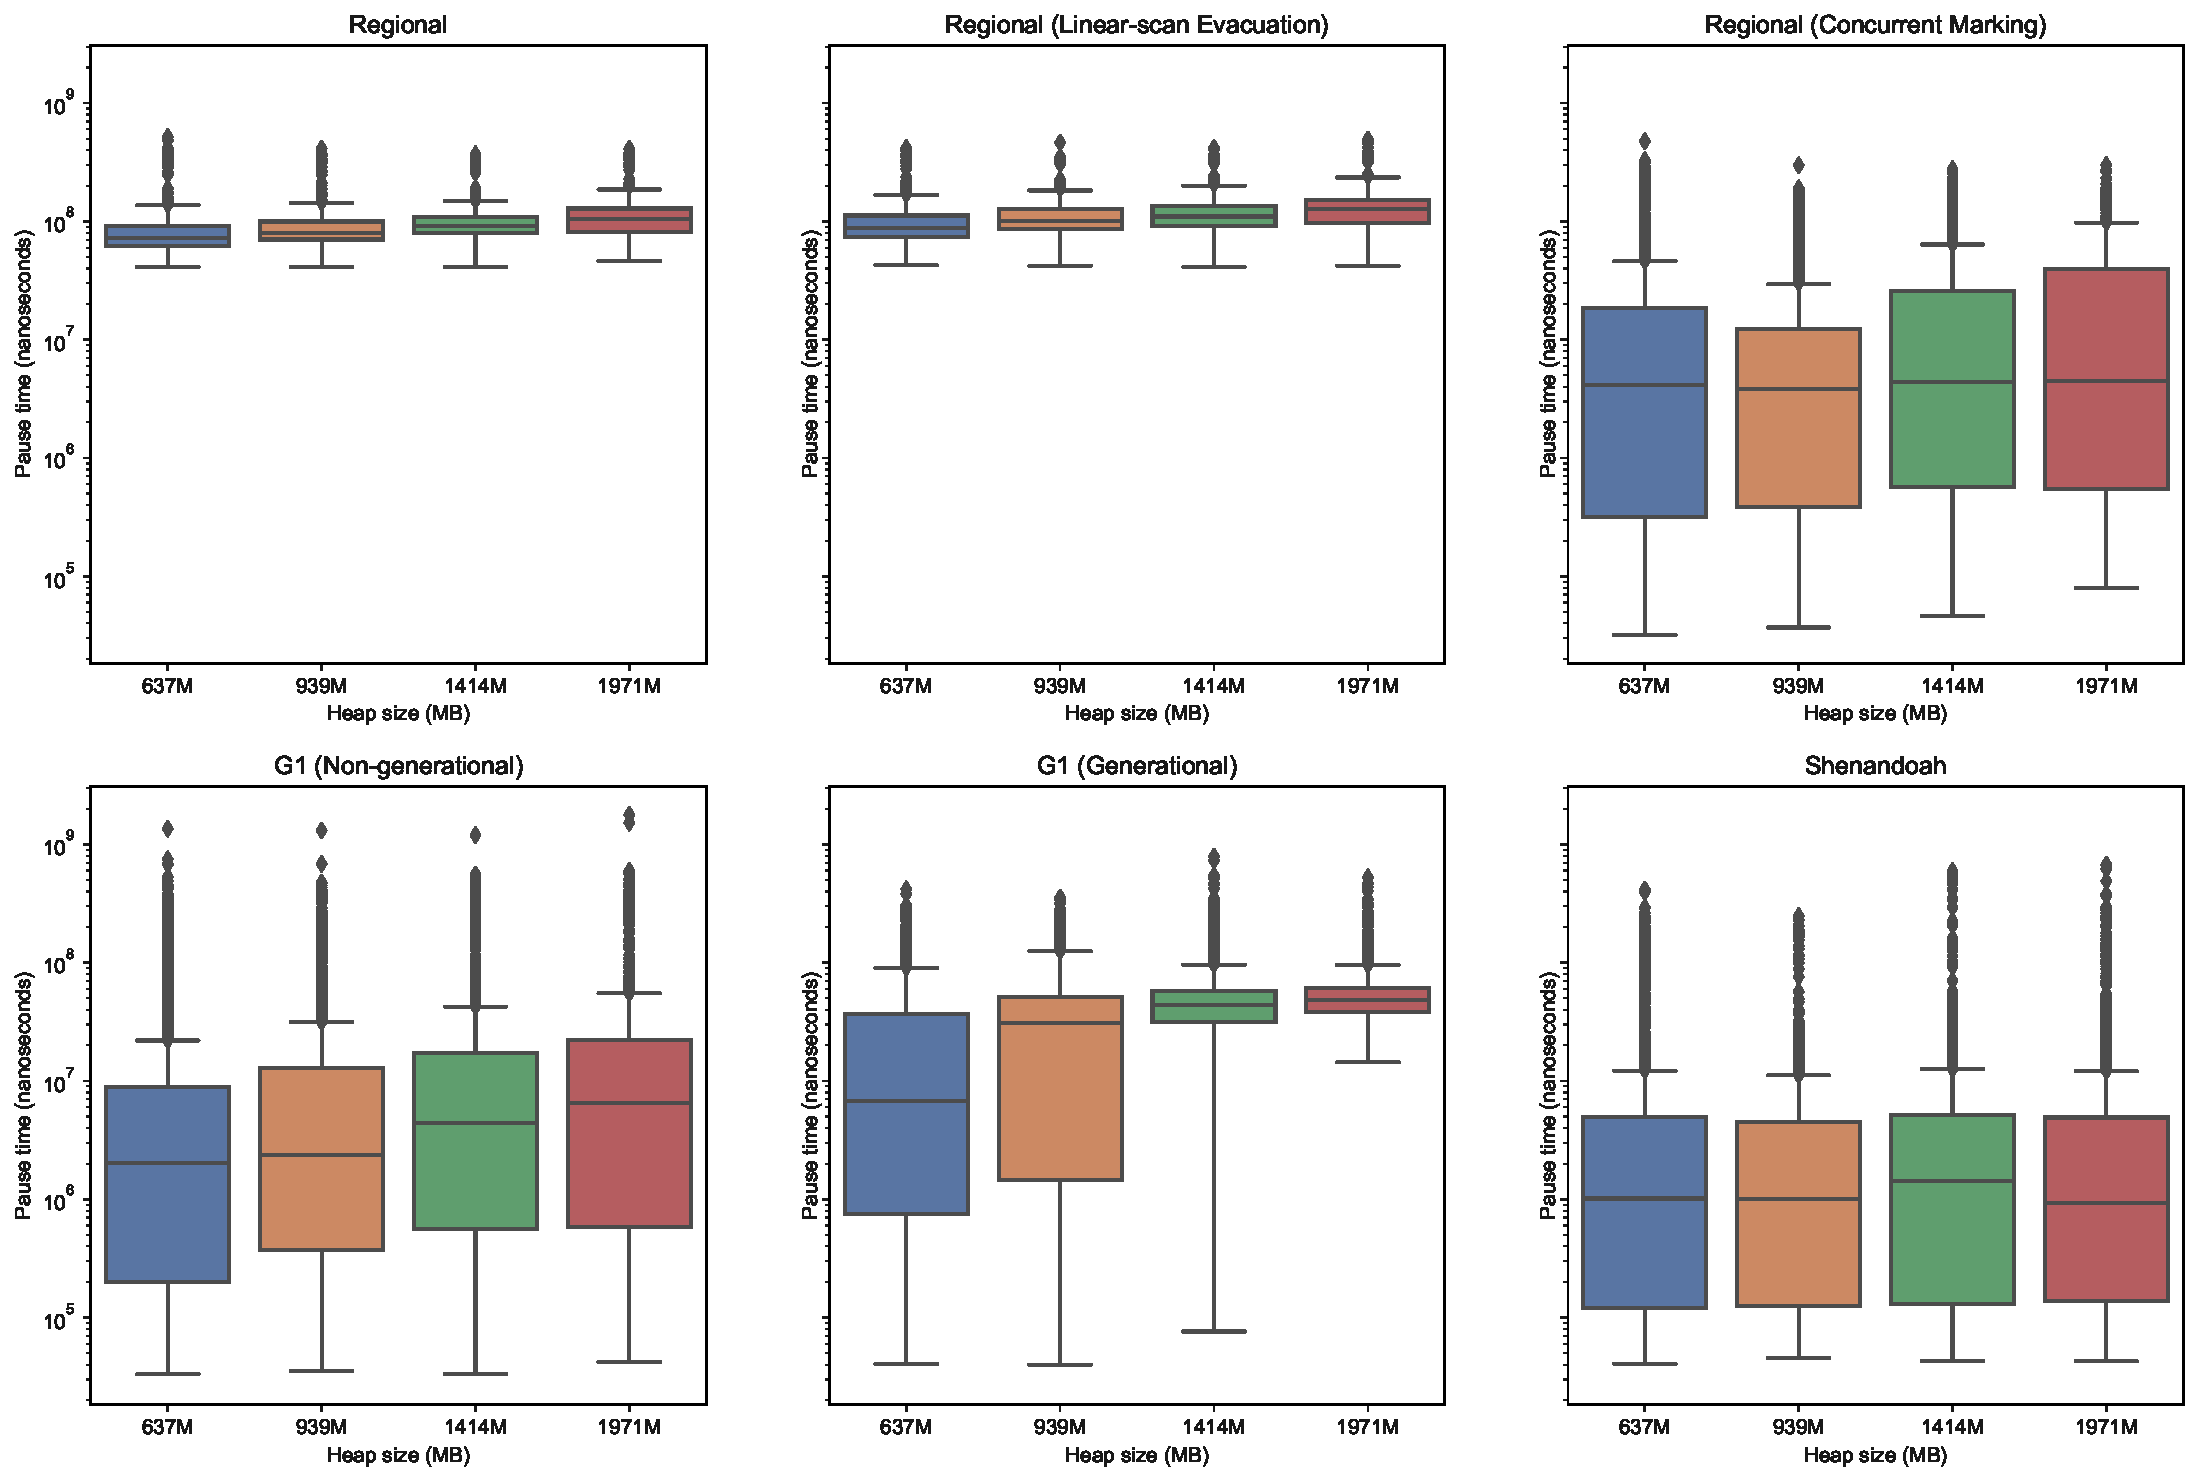
\includegraphics[width=\textwidth/1]{{figs/pause-time.pdf}}
  \caption{Pause times of 6 collectors}
  \label{fig:pausetime}
\end{figure*}

\begin{table*}
  \centering
  \input table/full-gc-ratio.tex
  \caption{Full GCs as a percentage of all GCs}
  \label{tab:fullgc}
\end{table*}

Table~\ref{tab:pause} shows the results of the GC latency time
evaluated on all 6 garbage collectors discussed in Section~\ref{cha:implementation}.
Specifically, the average, minimum, medium, 95\% percentile and maximum GC latency time nanoseconds
for each collector and each heap size,
as well as the overall GC latency time for each garbage collector
were reported.

To present the results more clearly, Figure~\ref{fig:pausetime} shows
the benchmarking results as a set of box plots with log-scaled pause time in nanoseconds as the y-axis.
Each subfigure shows the overall GC latency time for each garbage collection algorithm.

\subsection{Discussion}

As the most simple form of the G1 family of GC, the naive region-based collector, performs
stop-the-world GC during each GC cycle. Work for each GC cycle includes marking all
live objects and walking over the object graph to evacuate objects that are in a set of selected memory
regions. Two full heap tracings are performed during each GC cycle, which make the GC
pause time longer. The average pause time for this naive region-based GC generally ranges from $104$ to $147$
milliseconds and increases as the heap size increases.

By performing linear scan based evacuation, the linear-scan evacuation version of the region-based
GC perform a separate linear scan over the collection set
to evacuate live objects.
In this way, the collector generally has longer pause times,
which ranges from $110.1$ to $150.8$ milliseconds on average and increases as the heap size increases.
Linear scan evacuation increases the 95 percentile GC pause time by 15.8\%.
Although performing linear scan evacuation can increase the GC pause time,
this independent phase is an important component for G1 GC and the Shenandoah GC.

After performing concurrent marking in addition to the linear scan based evacuation,
the resulting concurrent-marking region-based collector splits the pause for marking into several smaller
pauses and performs most of the marking work concurrently without stopping the mutators.
This makes the total pause time for a GC smaller and significantly reduces the 95 percentile
GC pause time by 58.2\%.

The non-generational G1 reduces the collection size to meet a pause time goal of 100\,ms.
Based on the benchmarking results, at least 95\% of the pauses are less than the pre-defined
pause time goal. G1 uses remembered sets to update references
instead of performing a full heap tracing.
For heap sizes of 637\,MB, 939\,MB, 1414\,MB, and 1971\,MB, this
partial heap scanning technique reduces 95 percentile pause time by 30.4\%, 39.1\%, 47.7\% and 50.7\%
respectively. This reveals that the remembered sets based references updating has more benefits on
larger heaps. However, the full GC becomes more expensive because of the large work required
to update all the remembered sets in the heap, which usually results in a pause time
ranges from 0.5\,s to 1.0\,s.

By using the generational G1 GC, young/nursery GCs are usually triggered several times
before a major GC happens. Also, nursery GCs are fully stop-the-world and always tries
to collect as much nursery regions as possible, as long as the pause time does not exceed
the pre-defined pause time goal. This results in the increase of GC pause times.
However, the generational collection can largely reduce the probability of G1 GC falling
back to full GCs. As shown in Table~\ref{tab:fullgc}, I measured the overall number of full GCs a precentage of all GCs
for both non-generational and generational G1 GC on four different heap sizes,
with a 95\% confidence interval reported as well.
Based on the results, with the generational mode, G1 reduces the
probability of falling back to full GC by 12.5\%.

The Shenandoah GC performs marking, evacuation and reference updating concurrently,
this significantly reduces the pause time by 84.1\%, compared to the concurrent marking version
of the regional collector. Based on the benchmarking results at least 95\% of
the GC pauses do not exceed 18 milliseconds. However, full GCs can still result
in pauses of around 500 to 600 milliseconds, which are longer than the concurrent-marking
regional collector due to the Brooks barrier involved during the evacuation phase, which performance
will be discussed in Section~\ref{sec:barrierlatency}

\section{Concurrency overhead Evaluation} % 7
\label{sec:barrierlatency}

This section describes the steps took for concurrency overhead evaluation.
These concurrency overheads represent the mutator throughput reduction due to the
use of related concurrent algorithms (e.g. concurrent marking and evacuation).
This section also performs discussions of all the evaluation results.

\subsection{Methodology}

The concurrency percentage overhead is modeled as follows:
$$
\text{Overhead} = \frac{|\text{Concurrency overhead} - \text{Mutator time without the specific concurrent phase}|}{\text{Mutator time without the specific concurrent phase}} * 100\%
$$

The mutator execution time is calculated as the execution time of the benchmarking program with
stop-the-world GC time excluded.

As discussed in Chapter~\ref{cha:implementation}, I implemented the Garbage-first
family of collectors by performing progressive improvements over a simple region-based collector.
In this way, after performing an algorithmic improvement over a collector, we can measure the overhead of
the newly involved concurrent jobs or other technologies by comparing the benchmarking results
of the old collector and the new collector.

As an output of the analysis of the overhead data, the average Concurrency overhead
for each GC, each benchmark suite, each heap size and each concurrent phase this project used are reported
as well as their corresponding 95\% confidence interval.
The overall average overhead and its 95\% confidence interval for each concurrent job are also reported.

\subsection{Concurrent marking overhead}

\begin{table*}
  \centering
  \input table/satb-barrier.tex
  \caption{Concurrent marking overhead}
  \label{tab:satbbarrier}
\end{table*}

Table~\ref{tab:satbbarrier} shows the overheads of concurrent marking
as well as their 95\% confidence interval on different heap sizes.
Based on the evaluation data, the concurrent-marking
has an overhead of 22.0\% on average.

The SATB barrier used by the concurrent marking algorithm is a deletion barrier.
Furing concurrent marking, the barrier will trace and mark
all deleted nodes (i.e. the old object field when performing assignment \textjava{obj.x = y}) in the object graph.
A major difference between the SATB barrier used in these region-based collectors and
the concurrent mark-sweep GC is that the concurrent mark-sweep GC only marks objects
when tracing an object (the mark data is usually stored in the object header).
But the G1 family of collectors have to count the live bytes
for each region to assist with further collection set selection.
Also, these G1 family of collectors use off-heap mark table instead of object header to store
liveness data. For these reasons, a lot of atomic operations are involved during concurrent
marking which further reduces the mutator throughput, compared to the concurrent mark-sweep GC.
% The data shows that the SATB barrier increases the average mutator overhead by 92.93\%,
% which is an unignorable overhead. As a significant reason for causing such large overhead,
% all region-based

\subsection{Concurrent remembered-set refinement overhead}

\begin{table*}
  \centering
  \input table/remset-barrier.tex
  \caption{Concurrent remembered-set refinement overhead}
  \label{tab:remsetbarrier}
\end{table*}

Table~\ref{tab:remsetbarrier} shows the overheads of the Concurrent remembered-set refinement overhead
as well as their 95\% confidence interval on different heap sizes.

Node that this result represents the concurrency overhead of both remembered-set barriers and concurrent remset refinements.
The design of the remembered-set barriers and the remset refinement process follows
the original design of G1 that only 1 thread is used to process the dirty card
buffer and it only awakes for processing when the card buffer is full.

Based on the measurement results, the overhead of remembered-set refinement is not low,
which is 59.7\% on average. This is because the number of threads used for remset refinement
is not enough and the dirty card buffer always becomes full. Under such situation,
mutators have to take part of the responsibility to process cards in their local buffer,
which significantly reduces its throughput.

A possible fix, which has already been introduced into the OpenJDK's G1 implementation, is
to spawn more threads for remset refinement, and refinement threads can start processing cards earlier,
not necessarily need to wait until the global card buffer is full.

\subsection{Concurrent evacuation overhead}

\begin{table*}
  \centering
  \input table/brooks-barrier.tex
  \caption{Concurrent evacuation overhead}
  \label{tab:brooksbarrier}
\end{table*}

Table~\ref{tab:brooksbarrier} shows the overheads of the Concurrent evacuation overhead
as well as their 95\% confidence interval on different heap sizes.
On average, by using concurrent evacuation, the concurrency overhead of Shenandoah GC
is increased by 85.5\%.

This is a significantly high overhead. The reason for causing this is the use of 
"use barriers" which insert a barrier every time the JVM wants to access and use
an object reference. In addition, as described in Section~\ref{sec:shenandoahgc}, during the concurrent evacuation phase,
an extra barrier is used for every object comparison operation
to ensure the correct comparison between the forwarded and unforwarded pointer of the same object reference,
which further increases the concurrency overhead.

Another reason for causing this high overhead is that I could not fix a data race
problem happens during concurrent evacuation, due to the time scope of this project.
Instead I implemented a work-around to prevent this problem from happening.
This work-around has bad mutator performance since it requires addition
works (e.g. forward objects if necessary) to be done in read barriers.
Although the overhead of this work-around is not measured, it is expected to
contribute to most of the concurrent evacuation overhead shown in Table~\ref{tab:brooksbarrier}.
Plans to fix this problem will be discussed in Section~\ref{sec:future} as a part of the future work.

However, in order to perform concurrent evacuation and reference updating, the handling
of forwarded and unforwarded pointers is necessary.
One possible improvement is to use "colored pointers" to ensure the CPU will always access
the new version of the object pointer before using this pointer,
instead of go through the indirection pointer every time the mutator access the object.

\section{Remembered-Set Size} % 7
\label{sec:remsetsize}

As part of the evaluation of the G1 collector, I measured the remembered-set footprint
of G1 GC.

The implementation of remembered-set follows the design of the original OpenJDK
implementation, which uses a list of \textjava{PerRegionTable} as remembered-set
for each region. Each \textjava{PerRegionTable} remembers cards in one foreign region.
\textjava{PerRegionTable} is implemented as a bit table where each bit corresponds
to a card in the corresponding foreign region. 

Under such implementation, theoretically the space complexity for remembered-sets
is $O(N^2)$ where $N$ is the number of regions in the heap. Because each of total $N$ regions
has its own remembered-set and each remembered-set consists of $N-1$ \textjava{PerRegionTable}s
to remember cards in other $N-1$ regions. However, the practical space performance
of such remembered-set structure has never been formally measured.

Due to the same remembered-set structure,
measurements for the remembered-set footprint of JikesRVM's G1 implementation can reflect
the footprint of the OpenJDK's implementation, which can help us understand the
space performance of G1's remembered-sets under a real-world setting.

\subsection{Evaluation metrics}

In order to measure the remembered-set footprint carefully, two metrics are proposed
to reflect the space performance of remembered-sets:

\textbf{Committed Memory Ratio} is the ratio of the memory allocated for building remembered-sets
versus the total committed memory at some specific execution point.
This metric reflects the proportion of the heap that remembered-sets are actually take up.

$$ \text{Committed Memory Ratio} = \frac{\text{Committed memory for remset}}{\text{Total committed memory}} * 100\% $$

\textbf{Utilization Ratio} is the ratio of the memory (in bits) actually used for
remembered-sets to remember the cards, versus the total memory allocated for remembered-sets.
This metric reflects the proportion of the remembered-sets that is actually in use
and not be wasted.

$$ \text{Utilization Ratio} = \frac{\text{Bits actually used for store cards}}{\text{Committed memory for remset in Bits}} * 100\% $$

\subsection{Results \& discussion}

Remembered-set size is always changing during the execution of the program.
Plus, as the remembered-set refinement thread may still processing cards,
the remembered-set can be incomplete and may not remember all the corresponding cards.
Because in such situation some cards are still waiting to
be processed and write to some remembered-sets.

For this reason, I measure the remembered-set footprint at the start of each GC pause, immediately after
the stop-the-world remembered-set refinement is finished. At this time the remembered-set
footprint reaches a steady state, the remembered-set is complete and contains
all the corresponding cards under current heap state.

\begin{table*}
  \centering
  \input table/remset-size.tex
  \caption{Remembered set footprint}
  \label{tab:remsetfootprint}
\end{table*}

As shown in Table~\ref{tab:remsetfootprint}, I measured both proposed metrics
on both non-generational and generational G1 GC, with four different heap sizes.
For each kind of G1 GC and each heap size, I report the minimum value, maximum value and mean value
with 95\% confidence interval for both committed memory ratio and utilization ratio.

Based on the footprint data, we can see that for generational G1 Gc,
an average 9.6\% of the committed memory
is allocated for building remembered-sets, with a maximum proportion of 38.2\%.
For non-generational G1 GC the proportion of committed memory is 8.4\% on average.
Which means that remembered-sets are taking up too much memory in the heap. 
Also, the memory usage (i.e. utilization) for remembered-sets is pretty low,
only 2.3\% of the memory allocated for remembered-sets is actually used for remembering cards.
Taking the high committed memory ratio into consideration, this means that the
space efficiency of the \textjava{PerRegionTable} based remembered-sets is extremely
low. Hence a lot of optimization works should be done to further reduce the memory
waste of remembered-sets.

\section{Summary} % 2
\label{sec:summary}

This chapter discusses the measurement methodology and evaluation results of the
GC performance of the G1 family of garbage collectors. This includes the evaluation of
GC pause times and overhead of several concurrent phases. Also, the phenomenon revealed
in the measurement results is carefully discussed.

On the one hand, based on the measurement results, we can see that linear scan based evacuation
increases the work for each GC. Using concurrent marking, concurrent evacuation
or remembered set based partial heap scanning can significantly reduce the pause time
for each GC. On the other hand, using concurrent algorithms can largely increase the
mutator throughput reduction.

Also, based on the measurement results, the generational G1 and Shenandoah GC shows some
disappointing performances on GC pause time and concurrency overheads respectively.
However, the time scope of this project is limited.
In this way, there are still much optimization jobs and other works to do in the future,
which will be discussed in Chapter~\ref{cha:conc}.




%%% Local Variables: 
%%% mode: latex
%%% TeX-master: "paper"
%%% End: 


% We can also refer to specific lines of code in code listings. The bug in
% \Cref{fig:c:hello} is on \cref{line:bug}. There is also a bug in
% \Cref{fig:java:hello} on \crefrange{line:jbug-start}{line:jbug-end}. To
% achieve these references we put
% \texttt{(*@ \textbackslash label\{line:bug\} @*)}
% in the code -- the \texttt{(*@ @*)} are escape delimiters that allow you to add
% LaTeX in the (otherwise verbatim) code file.

% \begin{table*}
%   \centering
%   \caption{Processors used in our evaluation.  Note that the caption for a table is at the top.  Also note that a really long comment that wraps over the line ends up left-justified.}
%   \label{tab:machines}
%   \input table/machines.tex
% \end{table*}

% \begin{figure}
%   \centering
%   \begin{subfigure}[b]{\textwidth}
%       \lstinputlisting[linewidth=\textwidth,breaklines=true]{code/hello.c}
%       \caption{C}
%       \label{fig:c:hello}
%   \end{subfigure}

%   \begin{subfigure}[b]{\textwidth}
%       \lstinputlisting[linewidth=\textwidth,breaklines=true]{code/hello.java}
%       \caption{Java}
%       \label{fig:java:hello}
%   \end{subfigure}

%   \caption{Hello world in Java and C. This short caption is centered.}
%   \label{fig:helloworld}
% \end{figure}